\chapter{Uncertainties and Estimation}
\label{ch:UncertandEst}

We now have a robust method for the prediction of SM background for our search for the top squark. Along with a prediction for each of the backgrounds, we need to include the systematics uncertainties for our methods. Once we incorporate them we can confirm that our methods are correct by looking at the validation regions. Finally, we can then compare the final comparisons of data-to-simulation in our SR, which will allow us to set limits on the top squark mass. 

\section{Systematic Uncertainties}\label{sec:Uncert}
We will look at the various categories of systematic uncertainties that can affect the analysis. 
\begin{itemize}
	\item \textbf{Statistical uncertainty of control regions in data}: The dominant uncertainty in data-drivel background prediction methods is generally the result of limited statistics of the control regions that are used to derive the background estimate for the signal regions.
	\item \textbf{Statistical uncertainty of simulated samples}: In some cases, the uncertainties on transfer factors derived from simulation also have a significant statistical component due to limited statistics in the simulated samples.
	\item \textbf{Uncertainties related to extrapolation from control to signal regions}: Each data-driven background estimation method relies on an extrapolation from a control region to the signal region. This leads to uncertainties specific to each method, related to the nature of the extrapolation. For instance, the LL prediction strategy uses the region with a selected lepton to estimate the background yield in the vetoes region. Appropriate correction factors are applied to both selected and vetoes regions to account for differences in the lepton selection efficiency between data and simulation. The precision of these corrections affects the uncertainty in the background estimation. For the QCD prediction, we rely on an extrapolation from the low $\Delta\phi_{12}$ region, which is mostly in the core of the jet response distribution, to a region of high values of $\Delta\phi_{12}$, which is mostly in the tail of the distribution. We therefore assign an uncertainty in the QCD precition for the potential effects of severe jet mismeasurements in the jet response tails. 
	\item \textbf{Uncertainties related to $b$-tagging}: Effects related to the $b$-tagging are estimated to impact the scale factors up to 3\% for top-jets and between 5 to 10\% for \W+jets. Uncertainties due to the top-\pt{} reweighting, pile-up, or matching criteria results to effect smaller than 3\% for both top and \W{} tags. 
	\item \textbf{Uncertainties related to soft $b$-tagging}: The soft $b$-tagging methods are dependent on low-\pt{} jets and track reconstruction. The impact of these uncertainties are negligable for \ttbar{} and \W+jets and around 5\% for QCD events.
	\item \textbf{Uncertainties related to the merged top and W-tagging}: The impact of different effects on the determination of the scale factors are studied. One of the dominant sources is related to the description of the parton showering which results to uncertainties of 5-25\% and 8-15\%, for top and \W{} tagging, respectively. Another source of systematics is due to the modeling of the \ttbar{} topology. The evaluated uncertainties range between 1-3\% (1-12\%) in top (\W) tagging. 
	\item \textbf{Uncertainties related to the Resolved Top Tagging}: A similar list of the sources of systematic uncertainties is evaluated for the resolved tagger, as in the case of Merged tops. The most important sources stems from the description of the parton showering, which ranges between 8-31\%. The modeling of the \ttbar{} topology can be as high as 4\%, whereas potential dependence on the $b$-tagging results to uncertainties from 1 to 6\%. Uncertainties due to the top-\pt{} reweighting, pile-up, or matching criteria results to effect smaller than 3\%. 
	\item \textbf{Uncertainties related to lepton identification}: The control region of the LL is defined as having a single muon or electron. We must account for the acceptance and scale factor corrections for each particle. The impact is an approx. 1\%  and <1\% uncertainty for electrons and muons, respectively. It is also necessary to account for the misidentification of leptons (electrons, muons, and taus) that can contaminate our search region. 
	\begin{equation}\label{eqn:lepvetosyst}
		SF_{l}=1+\frac{N_l^{yield}-N_l^{SF}}{N_{SR}}
	\end{equation}
	This is shown in Eqn. \ref{eqn:lepvetosyst} where $N_l^{yield}$ and $N_l^{SF}$ are  the yield of simulation in the search region with a requirement of $N_l\geq1$ with and without the lepton scale factor and $N_{SR}$ is the yield in the search region with the lepton veto.  
	%\item \textbf{Luminosity}: A 2.6\% uncertainty is assigned on the integrated luminosity measured by CMS for the 2016 data-taking period. The prediction of the diboson backgrounds, which rely o simulaiton and are normalized based on the measured integrated luminosity, are affected by this uncertainty. Since the estimations of the remaining SM background processes are data-driven and based on the data observed in control regions, they are not affected by this uncertainty. 
\end{itemize}

\section{Validation}\label{sec:Validation}

\begin{table}[!ht]
\begin{center}
\caption[High $\Delta$m Search Regions]{\label{tab:validationregions-hm}Summary of the 151 disjoint search regions that mainly target high \dm~signal models. The high \dm~baseline selection is again $\nj \geq 5$, $\met>250~\GeV$, $\nb\geq1$, and $\dphijonetwothreefour>0.5$.}
\resizebox*{1\textwidth}{!}{

\begin{tabular}{|c|c|c|c|c|c|}
	\hline
	\multicolumn{6}{|c|}{$\mtb<175$\,\GeV}  \\
	\hline
	\nj				 & \nb				& \nt			   & \nw				 & \nrt				& \met~[\GeV] 		\\
	\hline
	$\geq7$		& $1, \geq2$  & $\geq0$		 & $\geq0$			& $\geq1$	  & $250-400,\geq400$ \\
	\hline
	\multicolumn{6}{|c|}{$\mtb\geq175$\,\GeV}  \\
	\hline
	\nj				 & \nb				& \nt			   & \nw				 & \nrt				& \met~[\GeV] 		\\
	\hline
	$\geq5$		& $1,\geq2$   &	$0$				& $0$				   & $0$			 & $250-400,\geq400$ \\
	\hline
	\multirow{4}{*}{$\geq5$} & \multirow{4}{*}{$1$} & $1$ & $0$ & $0$ & $250-400,\geq400$\\
						  &					   & $0$			 & $1$			& $0$			  & $250-400,\geq400$ \\
						  &					   & $0$			 & $0$				    & $1$	  & $250-400,\geq400$ \\
						  &					   & \multicolumn{3}{|c|}{$\nt+\nw+\nrt\geq3$} & $\geq400$ \\
	\hline
	\multirow{4}{*}{$\geq5$} & \multirow{4}{*}{$2$} & $1$ & $0$ & $0$ & $250-400,\geq400$\\
						  &					   & $0$			 & $1$					& $0$			& $250-400,\geq400$ \\
						  &					   & $0$			 & $0$				    & $1$	  		& $250-400,\geq400$\\
						  &					   & \multicolumn{3}{|c|}{$\nt+\nw+\nrt\geq3$} & $\geq400$ \\
	\hline
\end{tabular}
}
\end{center}
\end{table}

\begin{table}[!ht]
\begin{center}
\caption[Low $\Delta$m Search Regions]{\label{tab:validationregions-lm}Summary of the 53 disjoint search regions that mainly target low \dm~signal models. The low \dm~baseline selection is again $\nj \geq 2$, $\met>250~\GeV$, $\nt=\nw=\nrt=0$, $\nb\geq0$, $\mtb<175~\GeV$ (when applicable), $\pt(ISR) > 200$~\GeV, $ |\eta(ISR)| < 2.4$, $|\Delta\phi(j_{\text{ISR}},\met)|>2$, and $\metsig > 10$.}
\resizebox*{1\textwidth}{!}{
\begin{tabular}{|c|c|c|c|c|c|}
	\hline
	$\nj$              & $\nb$                    & $\nsv$             & $\ptisr$~[\GeV]         & $\ptb$~[\GeV]      & $\met$~[\GeV]                           \\
	\hline
	\multicolumn{6}{|c|}{\qcdlowdm}  \\
	\hline
	$2-5$              & \multirow{4}{*}{0}       & 0                  & \multirow{4}{*}{$\geq500$} & \multirow{4}{*}{-} & $250-400$ \\
	$\geq6$            &                          & 0                  &                         &                    & $250-400$ \\
	$2-5$              &                          & $\geq1$            &                         &                    & $250-400$ \\
	$\geq6$            &                          & $\geq1$            &                         &                    & $250-400$ \\
	\hline
	\multirow{5}{*}{$\geq2$} & \multirow{5}{*}{1}   & 0                  & $300-500$               & $20-40$            & $250-300$ \\
	&                          & 0                  & $300-500$               & $40-70$            & $250-300$ \\
	&                          & 0                  & $\geq500$                  & $20-40$            & $250-400$ \\
	&                          & 0                  & $\geq500$                  & $40-70$            & $250-400$ \\
	&                          & $\geq1$            & $\geq300$                  & $20-40$            & $250-300$            \\
	\hline
	$\geq2$            & \multirow{6}{*}{$\geq2$} & \multirow{6}{*}{$\geq0$} & $300-500$               & $40-80$            & $250-300$            \\
	$\geq2$            &                          &                          & $300-500$               & $80-140$           & $250-300$           \\
	$\geq7$            &                          &                          & $300-500$               & $\geq140$             & $250-300$            \\
	$\geq2$            &                          &                          & $\geq500$                  & $40-80$            & $250-400$            \\
	$\geq2$            &                          &                          & $\geq500$                  & $80-140$           & $250-400$            \\
	$\geq7$            &                          &                          & $\geq300$                  & $\geq140$             & $250-400$         \\
	\hline
	\multicolumn{6}{|c|}{\meddphi}  \\
	\hline
	$\geq2$			   & 0						& 0						   & $\geq200$					& $\geq20$			& $\geq250$		\\
	$\geq2$			   & 0						& 1						   & $\geq200$					& $\geq20$			& $\geq250$		\\
	$\geq2$			   & 1						& 0						   & $\geq200$					& $\geq20$			& $\geq250$		\\
	$\geq2$			   & 1						& 1						   & $\geq200$					& $\geq20$			& $\geq250$		\\
	\hline
	
\end{tabular}
}
\end{center}
\end{table}



In order to test and validate the background estimation strategy in data, we carry out the background estimation method in a lower \met{} region of the zero-lepton sample that is adjacent to the search sample, "low \met{} validation sample", and check the agreement between data and background prediction. The validaiton sample has significantly larger statistics than the search sample and is signal-depleted. Apart from the difference in the \met{} selection, the search selection on the other search variables is applied to the validation sample, with an exception of the regions with more than one top- or W-tags, where relaxed selections (i.e. drop selection in $M_T(b_{1,2},\met)$) are applied to gain more statistics, see Tables \ref{tab:validationregions-hm} and \ref{tab:validationregions-lm}. Figures \ref{fig:validation-region-lm} and \ref{fig:validation-region-hm} displays the SM estimate and the observed data in the different validation regions. Statistical uncertainties as well as systematic uncertainties resulting from the top- and W-tagging correction in the background predictions are shown in this plot. The data agrees well with the estimated backgrounds yields within uncertainties. 

\begin{figure}
	\begin{center}
  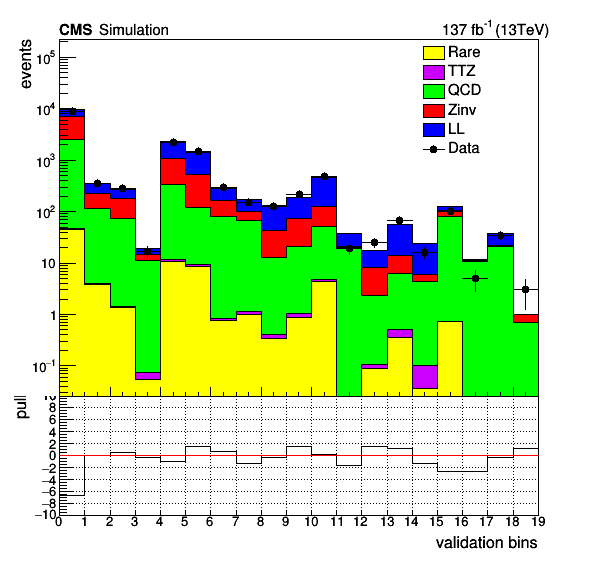
\includegraphics[width=1\textwidth]{validation_lowdm.png}
	\end{center}
	\caption[LM Validation Region]{Comparison of the data and SM backgrounds in the Low \dm{} validation regions.
	 }
	\label{fig:validation-region-lm}
\end{figure}

\begin{figure}
	\begin{center}
  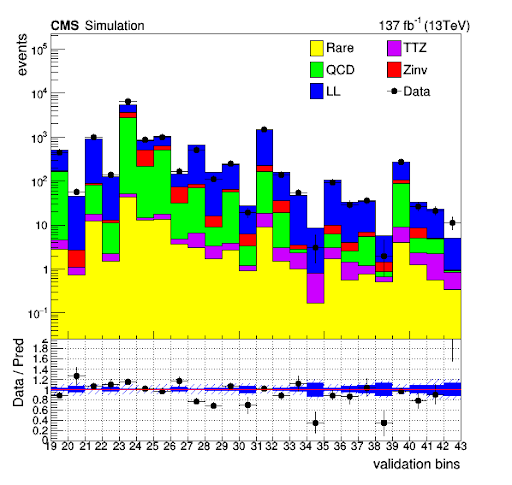
\includegraphics[width=1\textwidth]{validation_highdm.png}
	\end{center}
	\caption[Lost Lepton HM Control Region]{Comparison of the data and SM backgrounds in the High \dm{} validation regions.
	 }
	\label{fig:validation-region-hm}
\end{figure}

Now that we have shown that the bins for the low and high \dm{} match well with data we can move to a full comparison of the data and simulation in the SR. To do this we combine the predictions from the LL, \Znunu, QCD, and Rare backgrounds. We need to 

\section{Combination of Search region}\label{sec:Combination}

As we have seen, this analysis has quite a large parameter space of interesting mass points. This combined with the number of SR bins and different backgrounds in each bin it is necessary to discuss how we plan of combining all of this to get a final estimation. To do this we use a datacard method to perform the combination and uncertainty calculation for our counting experiment. In Fig. \ref{fig:example-datacard-sig}, we have an example of a single bin from our SR, specifically bin 61 (high $\dm, \nb=1, \mtb\geq175, \nt=0, \nrt=0, \nw=0, \Ht\geq1000, 250\leq\met<350$), for a single signal sample, T2tt(175, 1). 

Let go through Fig. \ref{fig:example-datacard-sig}, so that we can understand what is going on. The parameter \textit{imax} is the number of final states analyzed in the datacard, \textit{jmax} is the number of independent physical processes whose yields are provided minus 1, and \textit{kmax} is the number of independent systematic uncertainties. Here we put "*" and allow the computation to figure that out. Next, we have the number of observed events from data in this particular bin, shown as \textit{observation}, where the bin above it is a unique name. Then, in the five lines following, we have the yields for the different processes included in this bin. The first process denoted as \textit{signal} is the yield from T2tt(175,1), then the other four processes are the SM backgrounds in this bin. 

\begin{figure}
	\begin{center}
  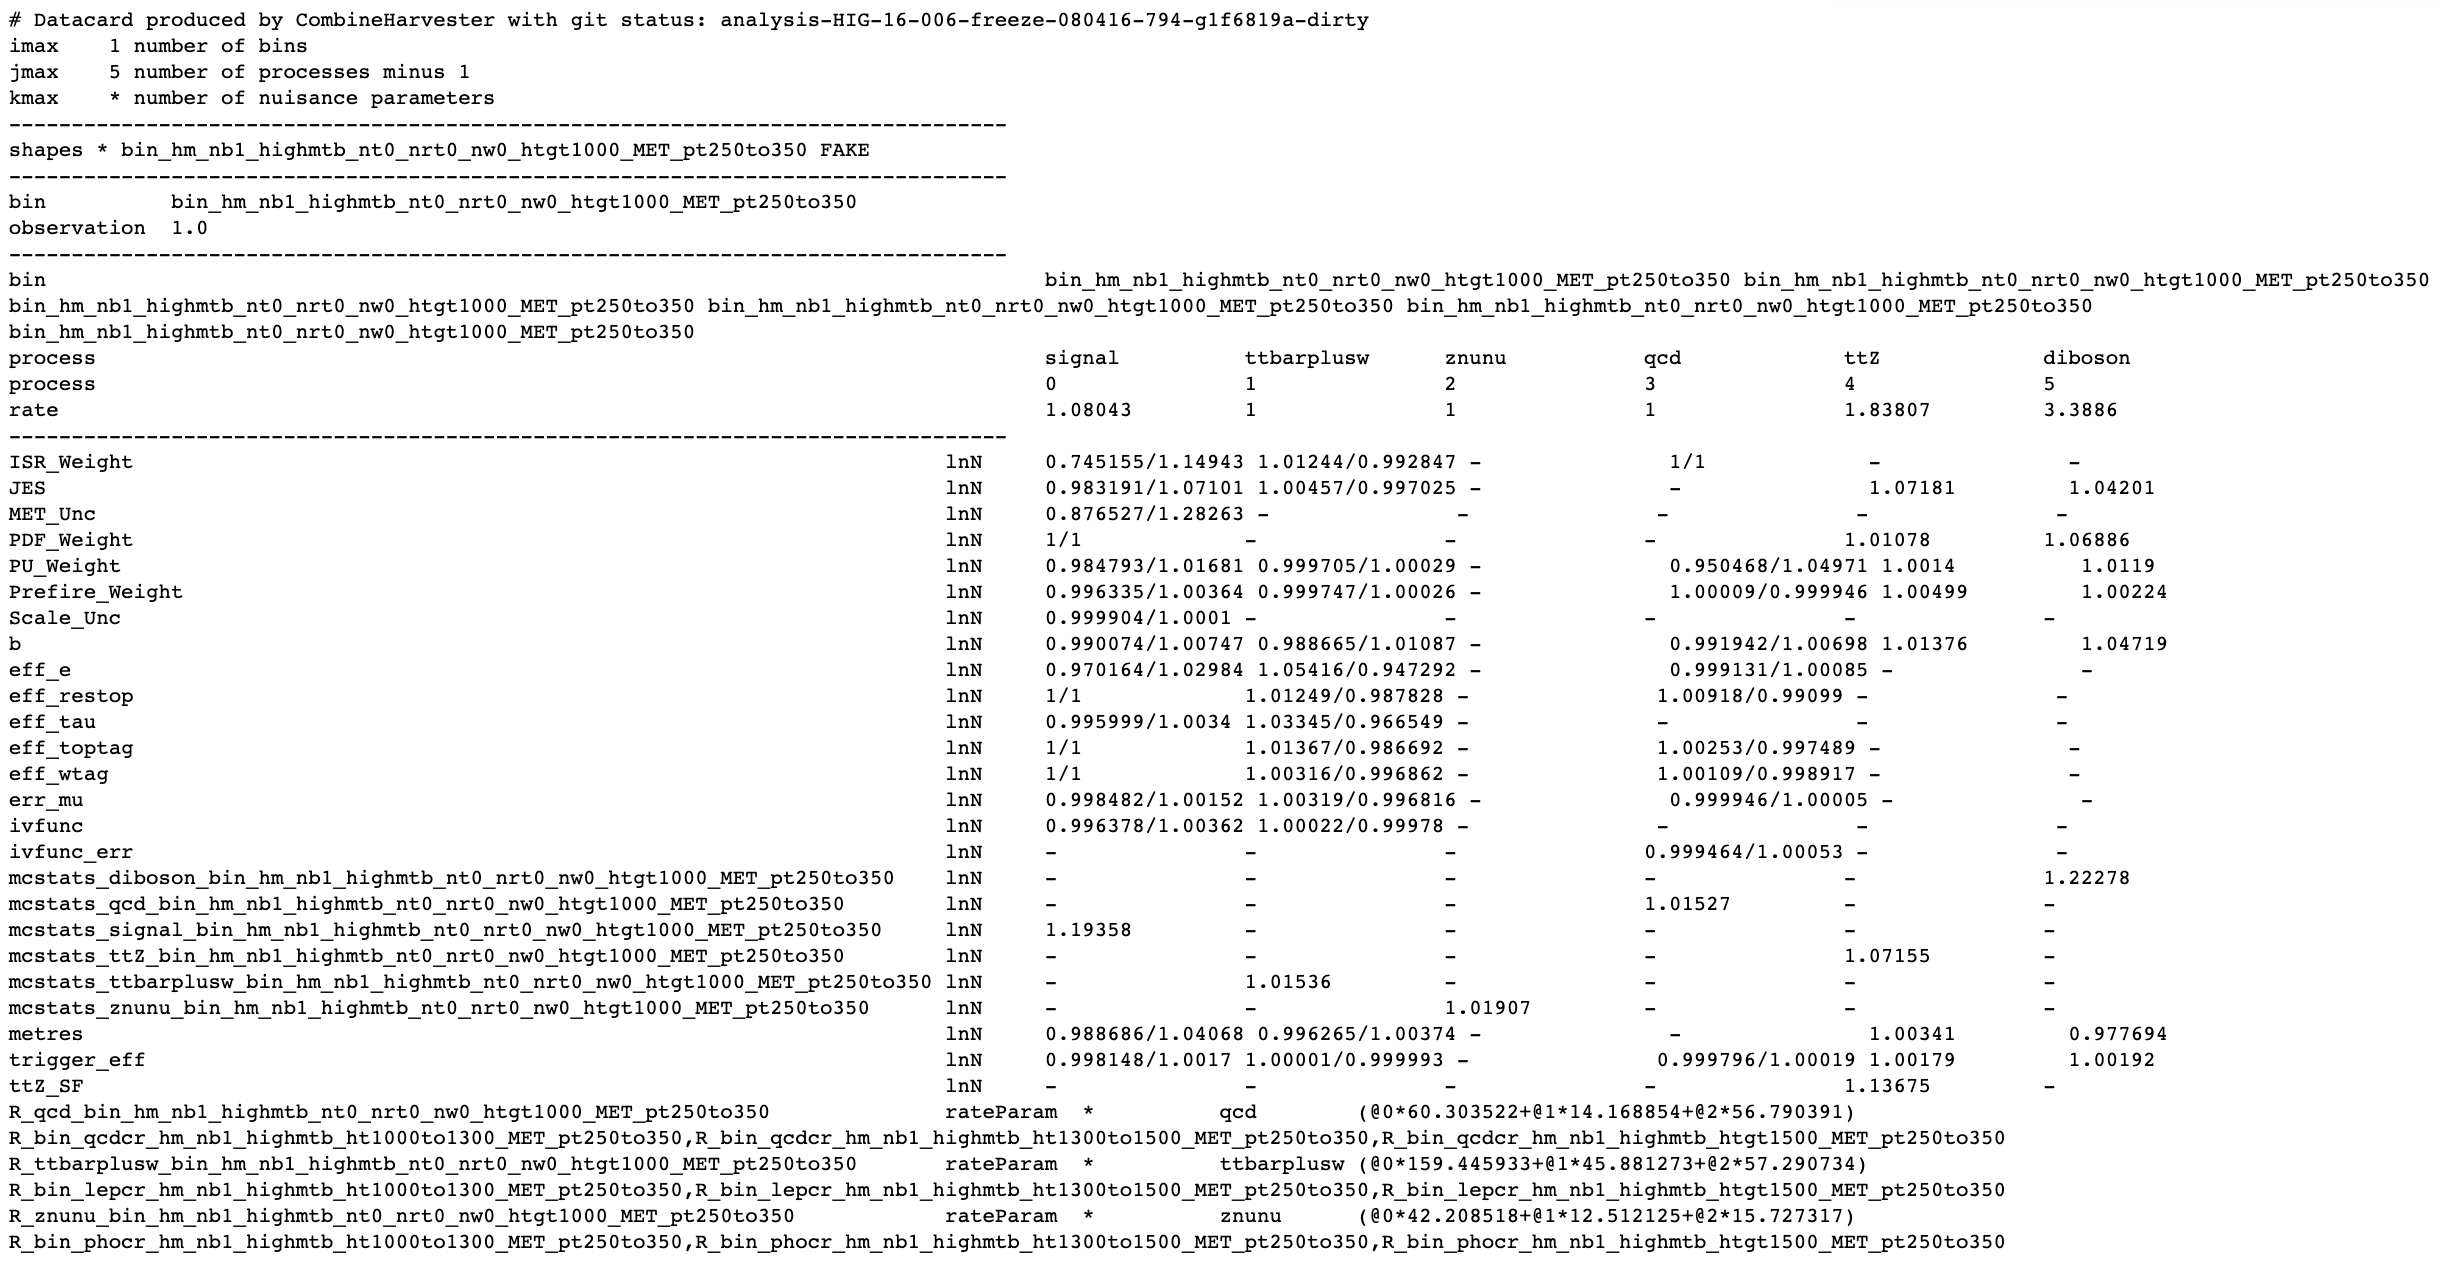
\includegraphics[width=1\textwidth]{T2tt_175_1_example_bin_hm_nb1_highmtb_nt0_nrt0_nw0_htgt1000_MET_pt250to350.png}
	\end{center}
	\caption[Example Datacard of T2tt(175,1)]{An example of the datacard for a single bin of T2tt(175,1) with background and uncertainties.
	 }
	\label{fig:example-datacard-sig}
\end{figure}
\begin{figure}
	\begin{center}
  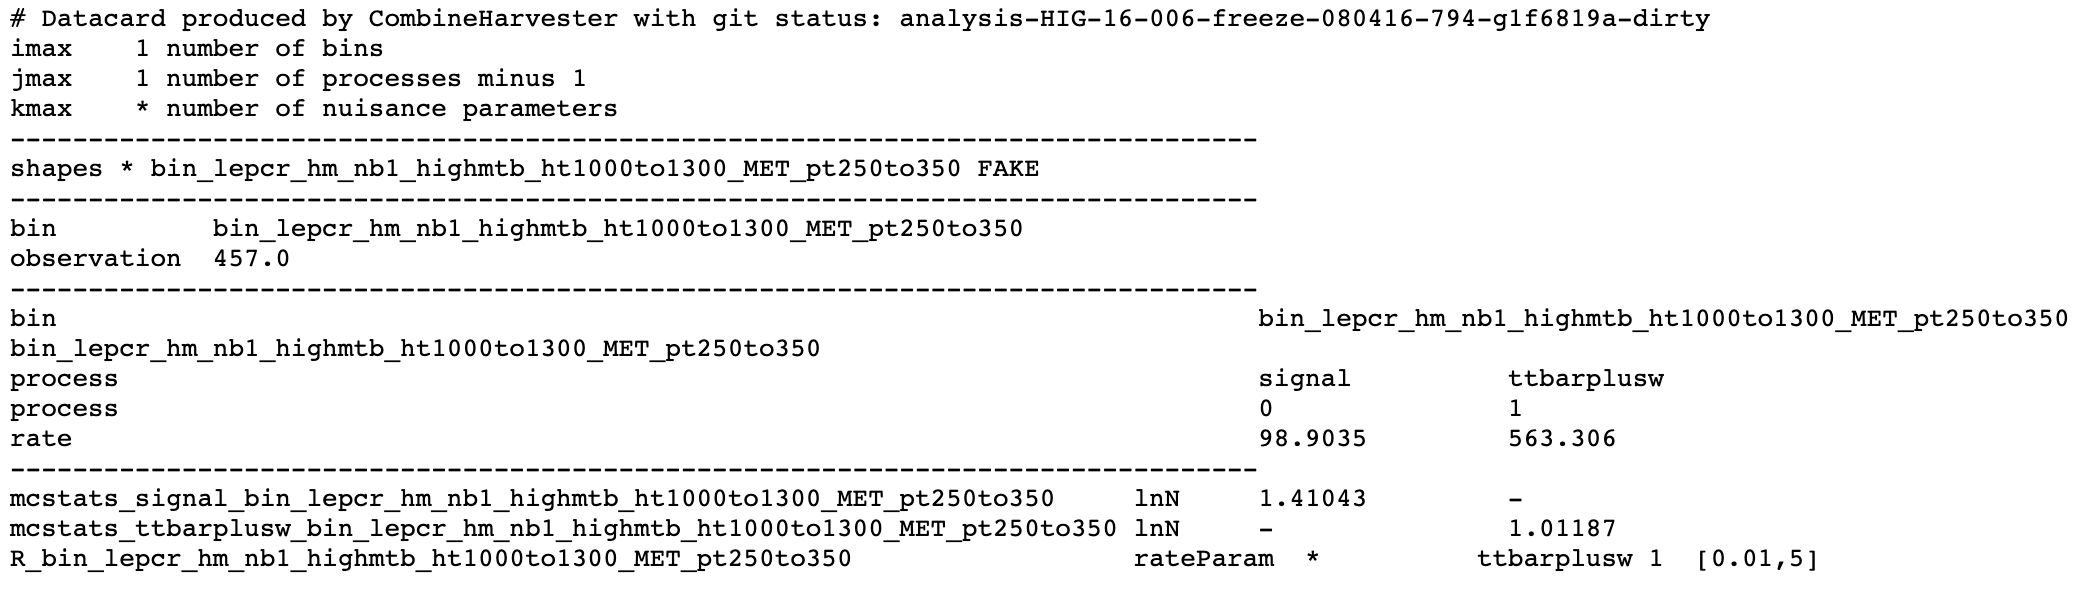
\includegraphics[width=1\textwidth]{bin_lepcr_hm_nb1_highmtb_ht1000to1300_MET_pt250to350.png}
	\end{center}
	\caption[Example Datacard of LL CR]{An example of the datacard for the LL CR with signal contamination.
	 }
	\label{fig:example-datacard-ll}
\end{figure}
\begin{figure}
	\begin{center}
  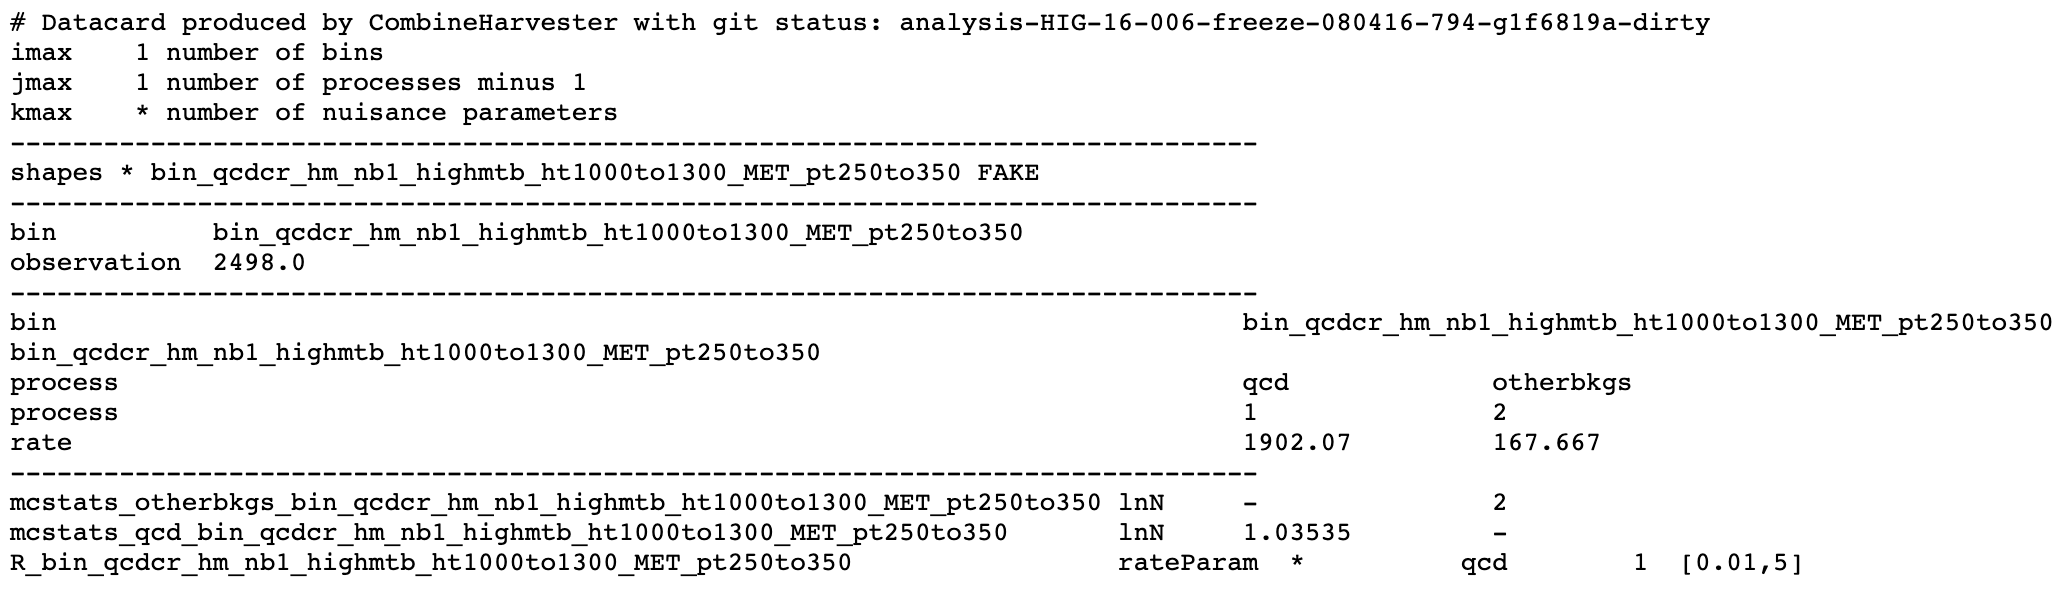
\includegraphics[width=1\textwidth]{bin_qcdcr_hm_nb1_highmtb_ht1000to1300_MET_pt250to350.png}
	\end{center}
	\caption[Example Datacard of QCD CR]{An example of the datacard for the QCD CR.
	 }
	\label{fig:example-datacard-qcd}
\end{figure}

The next major portion of the datacard is the various systematics of the signal and background processes. The most common type of uncertainty is the log-normal which is denoted by \textit{lnN}. For these, the distribution is described by the parameter $\kappa$, which is a multiplicative error. A $+1\sigma$ deviation corresponds to a yield scaled by $\kappa$ while a $-1\sigma$ scales the yields by $\frac{1}{\kappa}$. If the uncertainties are small the log-normal error can be approximated by a gaussian and we can approximate $\kappa=1+\frac{\delta x}{x}$, where $\frac{\delta x}{x}$ is the relative uncertainty of the event yield. Each process has a value for the statistical uncertainty which is a poisson error of $\sqrt{N}$. Then each process can have a systematic error that may be correlated to other backgrounds. In each process, we can have a value for the uncertainty or a dash which means that the uncertainty does not contribute to the process. 

Finally at the bottom of the datacard we have the rate parameters for the backgrounds that require the extrapolation from units to SR bins. The units are a more basic definition of the SR bins that can be combined with the prediction of each background to give the total background in each SR bin. Since the LL, QCD, and \Znunu{} backgrounds use an extrapolation method for the high \dm{} bins, we have defined 112 CR units and 529 SR units. In the bottom of Fig. \ref{fig:example-datacard-sig}, are the expected rates for the LL, QCD, and \Znunu{} that show the combination of three units to give the prediction of each background in the respective bins. The rates from the LL and QCD background can be seen in Fig. \ref{fig:example-datacard-ll} and \ref{fig:example-datacard-qcd}. These are an example of a single unit datacard. The calculation for each background from the unit CR is the data observation divided by the SM background in each, $\frac{N_{data}^{CR}}{(N_{LL}^{CR} + N_{Sig}^{CR})}$ where the LL CR is used as an example. Now to be able to make the estimation of the limit for the various SUSY processes that we are looking at, we need to combine the datacards for each SR bin for all of the signals in the mass parameter space. This can be easily accomplished thanks to the unique bin and process names for each signal. We can then input each of these combined datacards into the Higgs Combined Tool.

\section{Statistics}\label{sec:Statistics}

For the combination of multiple analyses that are sensitive to different signal production mechanisms and different decay modes, we are required to set limits on a common signal strength modifier $\mu$ that is used to alter the cross sections of all the production mechanisms. 

\section{Higgs Combined Tool}\label{sec:HiggsCombined}

The Higgs Combined Tool \cite{noauthor_procedure_2011} uses a modified frequentist method to compute the confidence level (CL) \cite{read_presentation_2002, junk_confidence_1999, read_modified_2000} for each of the cross section limits. The tool is able to convert the datacards into a Likelihood function to calculate the limits. The Likelihood function is 
\begin{equation}\label{eqn:likelihood}
\mathcal{L}(\mu,\theta)=\prod_i \frac{[\mu\cdot s_i(\theta)+b_i(\theta)]^{n_i}}{n_i !}e^{-[\mu\cdot s_i(\theta)+b_i(\theta)]}\prod_\kappa e^{-\frac{1}{2}\theta^2_\kappa},
\end{equation}
where $\mu$ is the POI which is constrained only by the observed data, $s_i(\theta)$ and $b_i(\theta)$ are nuisance parameters for signal and background. Both the signal and background are subject to multiple uncertainties that are dealt with by using nuisance parameters $\theta$. Each of these three parameters are jointly fitted to get a value of $\mu$. We will be using an asymptotic CL method to compute the limits for this analysis. 

\subsection{Observed Limits}\label{sec:ObsLimits}

To compute the observed limit the likelihood function, $\mathcal{L}(\mu,\theta)$ from Eqn. \ref{eqn:likelihood}. Comparing the compatability of the data with the background-only and signal+background hypotheses to get 
\begin{equation}
\widetilde{q}_\mu=-2 ln\frac{\mathcal{L}(\mu,\hat{\theta}_\mu)}{\mathcal{L}(\mu,\theta)},
\end{equation}
with a constraint $0\leq\hat{\mu}\leq\mu$ where $\hat{\theta}_\mu$ is the conditional maximum likelihood estimators of $\theta$ given the signal strength $\mu$ and data, and the estimators $\hat{\mu}$ and $\hat{\theta}$ are the global maximum of the likelihood. 

From this, we get the observed value of $\widetilde{q}_\mu^{obs}$ for a given value of $\mu$. A toy Monte Carlo pseudo-data is used to construct the PDFs $f(\widetilde{q}_\mu|\mu,\hat{\theta}_\mu^{obs})$ and $f(\widetilde{q}_\mu|0,\hat{\theta}_0^{obs})$ where we have a signal with strength $\mu$ in the signal+background and a background-only hypothesis. Two $p$-values are defined and associated with the two hypotheses, $p_\mu$ and $p_b$,
\begin{equation}\label{eqn:splusb}
p_\mu=P(\widetilde{q}_\mu\geq\widetilde{q}_\mu^{obs}|\text{signal+background})=\int_{\widetilde{q}_\mu^{obs}}^{\infty}f(\widetilde{q}_\mu|\mu,\hat{\theta}_\mu^{obs})d\widetilde{q}_\mu,
\end{equation} \label{eqn:b}
whe then have
\begin{equation}
1-p_b=P(\widetilde{q}_\mu\geq\widetilde{q}_\mu^{obs}|\text{background-only})=\int_{\widetilde{q}_\mu^{obs}}^{\infty}f(\widetilde{q}_\mu|0,\hat{\theta}_0^{obs})d\widetilde{q}_\mu,
\end{equation}
using both of these we can calculate the $CL_s(\mu)$ as 
\begin{equation}
CL_s(\mu)=\frac{p_\mu}{1-p_b}.
\end{equation}
Finally, to quota a $95\%$ confidence level on the upper limit on $\mu$, $\mu$ is adjusted until the $CL_s=0.05$ such that the confidence level is $(1-\alpha)$ where $CL_s\leq\alpha$. 

\subsection{Expected Limits}\label{sec:ExpLimits}

Along with the observed limits we are also interested in calculating the expected median upper-limit, $\pm1\sigma$, and $\pm2\sigma$ bands for the background-only hypothesis. To do this we generate a large set of background-only pseudo-data, using the toy Monte Carlo method, and calculate the $CL_s$ as if it was real data. The calculation for the expected limit is done by finding the cumulative probability distribution function (CDF) of results and starting the integration. The point at which the CDF crosses the 50\% band is the median expected value. Then the $\pm1\sigma$ band is defined by the 16\% and 84\% band and the $\pm2\sigma$ band is the 2.5\% and 97.5\% crossings. 